\documentclass[11pt]{article}
\usepackage[T1]{fontenc}
\usepackage{lmodern}
\usepackage[margin=1in]{geometry}
\usepackage{amsmath,amssymb}
\usepackage{graphicx}
\usepackage{booktabs}
\usepackage{array}
\usepackage{float}
\usepackage{xcolor}
\usepackage[hidelinks]{hyperref}

\setlength{\parskip}{0.45em}
\setlength{\parindent}{0pt}
\newcommand{\xs}{x^{*}}

\title{\vspace{-3.2em}How uncertain is a posterior-predictive 1-in-100-year level?\\
\large A synthetic-data check of the M\"uller--Watson Bayesian model}
\author{Produced by Ken Caldeira with the help of Claude Code \\ \small\url{https://github.com/Sustainable-Solutions-Lab/extreme-trend-detection}}
\date{Preliminary note, 4 November 2026}

\begin{document}
\maketitle
\vspace{-2.0em}

\section*{Summary}

\emph{The question.} A 1-in-100-year level can be read off a Bayesian model of time-varying
extremes in two ways. One takes a statistic (median or mean) of the 99th percentiles implied by
the individual posterior draws. The other, which we call \emph{the predictive level}, first
averages the draws' distributions into one posterior predictive distribution and then takes its
99th percentile. The predictive level is a single, well-defined number, and it is the one a
learner who holds the posterior should use to price a contract that pays when the level is
exceeded. We asked how close that number is to the truth, and where its uncertainty comes from,
using synthetic records whose true risk is known exactly.

\emph{What we did.} We fitted the four-random-walk GEV model of M\"uller and Watson (2024), with
the authors' code and priors, to synthetic records of annual maxima (30, 45 or 85 years)
drawn from four daily distributions (19,700 model fits), including a precipitation-like gamma distribution, with
and without known changes in their mean, spread or tail. In each record we computed the predictive
99th percentile for the final year and asked how often that level is truly exceeded.

\emph{On average across records the predictive level is about right or conservative.} The true
chance of exceeding it averages 0.85\% at 85 years and 0.4--0.6\% at 30--45 years, against the
1\% it is meant to have, whereas the posterior median and the maximum-likelihood fits average
1.6--3.7\%. It rarely understates the risk (13\% of records at 85 years, 6--8\% at 30--45 years, against
30--40\% for the other estimators).

\emph{In a single record it usually overstates the risk, and often by a lot.} The median true
chance of exceeding it is 0.39\% at 85 years, 0.05\% at 45 years and 0.01\% at 30 years: the
level reported as the 1-in-100-year event is typically a 1-in-250, 1-in-2,000 and 1-in-10,000-year
event. It is off by more than a factor of 2 in either direction in 68\%, 84\% and 92\% of records,
9 to 19 percentage points more often than the posterior median or a simple trend fit. In the
precipitation-like case, the predictive 100-year depth is typically 8\% (85 years), 22\% (45) and
31\% (30) above the true one, and in one record in ten more than 25\%, 66\% and 138\% above.

\emph{As a price, it is conservative and very variable.} For cover whose true risk is 1\% a year,
the model's predictive probability, its pure premium rate, has a median of 1.7\% at 85 years and
2.8--3.2\% at 30--45 years. It is rarely below 0.5\% (4--10\% of records), whereas a location-trend
fit underprices by more than a factor of 2 in 36--45\% of records and by more than a factor of 10
in 16--28\%.

\emph{The uncertainty comes from the short record and the prior, not from the computation.}
\begin{itemize}\setlength{\itemsep}{1pt}
\item Across equally plausible records of the same climate, the true chance of exceeding the
  predictive level spans a factor of about 160 at 85 years (10th to 90th percentile 0.015\% to
  2.4\%), and far more at 30--45 years.
\item Within a record, the posterior itself is very uncertain about the risk at that level: the
  typical draw puts it at 0.2\% (85 years) or essentially 0\% (30 years), while the top 5\% of
  draws put it above 4.6--5.8\%. The 1\% is an average over beliefs that range from almost nothing
  to five or more times the target. The top 5\% of draws carry 38--52\% of it.
\item The overstatement is largest in records whose posterior leans towards heavy tails (a
  GEV shape $\xi$ well above zero), heavier than in any of our synthetic climates
  ($\xi\lesssim0.2$).
\item Shrinking the prior scales of the random walks (a ``tight prior'') lowers the predictive
  level, raises its typical true exceedance from 0.39\% to 0.64\% at 85 years and from 0.05\% to
  0.24\% at 45 years, and brings its accuracy close to that of the posterior median.
\item Monte Carlo error is negligible: with 4,000 draws it changes the exceedance probability by
  about 5--10\%, and with the authors' 40,000 draws by 2--3\%; it is well under 1\% of the error
  variance.
\end{itemize}

\emph{Most of the ambiguity is there even when nothing is changing.} In records from a stationary
climate the predictive level is just as dispersed and just as high: it misses by more than a factor
of 2 in 64\%, 80\% and 89\% of records at 85, 45 and 30 years. The high and volatile risk
estimates come mainly from estimating a heavy upper tail from a few decades of data under a prior
that allows very heavy tails, not from non-stationarity as such.

\emph{What we would suggest.} Report, beside the predictive level, how the posterior's beliefs
about the risk at that level are spread (e.g.\ the median draw and a 90\% range); show how the level
moves under a tighter prior on the random walks and on $\xi$; fit the same model to stationary
synthetic records of the same length to see how much ambiguity arises with no change at all; and
use pooled regional information on the tail shape where possible (Section~\ref{sec:suggest}).

\tableofcontents

\section{What we tested}\label{sec:what}

\subsection{The predictive level}

The model gives, for each posterior draw $d=1,\dots,D$, GEV parameters
$\theta_d(t)=(\mu_d(t),\sigma_d(t),\xi_d(t))$ for the annual maximum in year $t$. The draw's own
99th percentile is $q_d(t)$, with $P(Y_t>q_d(t)\mid\theta_d)=1\%$. The \emph{posterior median}
estimate is the median of the $q_d(t)$ over draws. The \emph{predictive level} $\xs(t)$ instead
solves
\begin{equation}
\frac1D\sum_{d=1}^{D} P\bigl(Y_t>\xs(t)\mid\theta_d(t)\bigr)=1\%,
\end{equation}
the 99th percentile of the posterior predictive distribution of the year-$t$ maximum. It averages
probabilities, not levels. Since a probability cannot go above 1 but can fall to zero, and the
upper tail of a GEV distribution is very sensitive to $\xi$, the average is pulled up by the draws
with the heaviest tails: in our records $\xs$ is above the posterior median in every record, and
above the posterior mean of $q_d$ in two-thirds of records at 85 years (a tenth at 30 years;
Figure~\ref{fig:anatomy}).

We assume that the reported ``99th percentile of the posterior rainfall distribution'' is this
predictive 99th percentile of the annual-maximum distribution, i.e.\ the 1-in-100-year level, in
the final year of the record. If it is a percentile of another quantity (daily rainfall, say), the
mechanism below still applies but the numbers will differ.

\subsection{The model, the data and the score}

\begin{description}\setlength{\itemsep}{1pt}
\item[Model] The four-random-walk GEV model of M\"uller and Watson (2024), their Stan code and
  priors unchanged (random walks in $\xi$ and in three scale and location terms; innovation scales
  $\gamma=\mathrm{sg}\cdot g/\sqrt T$ with $g\sim\mathrm{Exp}(1)$ and $\mathrm{sg}=1, 0.5, 0.5$; $\xi$
  confined to $(-0.9, 2.1)$). Four chains of 1,000 warm-up and 1,000 sampling iterations
  (\texttt{adapt\_delta} 0.95). The ``tight prior'' runs use $\mathrm{sg}=0.25$ for all three.
\item[Data] Daily series with day-to-day correlation 0.5 (0 in one design) from four distributions:
  normal (temperature-like), gamma with shape 2 (precipitation-like), Student-$t$ with 6 degrees of
  freedom (heavy-tailed) and a bounded beta. We fitted the annual maxima (or the three largest
  values per year, declustered, in the ``3/yr'' designs). Each distribution was left unchanged or
  had its mean, spread, tail or (beta) position changed linearly or in a step; further cases make
  the spread and tail follow a rising mean, as a covariate model would assume, or change linearly
  in time between the same end points. Each case has 100 records.
\item[Truth] Because the generating process is known, so is the true distribution of the final
  year's annual maximum, and with it the true chance of exceeding any reported level.
\item[Score] A reported 1-in-100-year level \emph{understates} the risk by more than a factor of 2
  if its true chance of being exceeded is above 2\%, and \emph{overstates} it if that chance is
  below 0.5\%. We call the sum the share \emph{missed}.
\item[Comparison] The same records were scored with the posterior median and mean of $q_d$, a
  maximum-likelihood GEV fit with a linear trend in location, and an Akaike-weighted average of
  four simple fits (constant, location trend, location and width trend, mean-state covariate).
  Because all estimators see the same records, differences between them are measured to about
  $\pm1.5$ percentage points.
\end{description}

\section{How close is the predictive level to the truth?}\label{sec:close}

Table~\ref{tab:designs} and Figure~\ref{fig:exceedance} give the main result, pooled over the
standard cases (the four distributions with and without change).

\begin{table}[H]
\centering\small\setlength{\tabcolsep}{3.5pt}
\caption{True chance of exceeding the reported 1-in-100-year level in the final year, standard
cases (2,000 records per design). For the predictive level: median and average over records, and
the shares (\%) understated ($>2\%$) and overstated ($<0.5\%$) by more than a factor of 2. Right:
the share missed by the other estimators on the same records, and the difference predictive minus
posterior median ($\pm$ one standard error).}\label{tab:designs}
\begin{tabular}{l rrrrr rrr r}
\toprule
 & \multicolumn{5}{c}{Bayes, predictive} & \multicolumn{3}{c}{Missed, others} & \\
\cmidrule(lr){2-6}\cmidrule(lr){7-9}
Design & median & avg. & under & over & \textbf{missed} & \shortstack{post.\\median} & \shortstack{loc.\\trend} & \shortstack{AIC\\avg.} & \shortstack{pred.\ $-$\\median} \\
\midrule
30 yr & 0.01\% & 0.5\% & 8 & 84 & \textbf{92} & 75 & 73 & 75 & $+17\pm1$ \\
45 yr & 0.05\% & 0.4\% & 6 & 78 & \textbf{84} & 70 & 69 & 69 & $+14\pm1$ \\
85 yr & 0.4\% & 0.8\% & 12 & 56 & \textbf{68} & 59 & 56 & 51 & $+9\pm2$ \\
85 yr, 3/yr & 0.5\% & 0.9\% & 13 & 53 & \textbf{66} & 55 & 55 & 46 & $+11\pm2$ \\
85 yr, indep. days & 0.3\% & 0.8\% & 13 & 58 & \textbf{71} & 65 & 58 & 55 & $+6\pm2$ \\
45 yr, tight prior & 0.2\% & 0.7\% & 11 & 63 & \textbf{74} & 70 & 69 & 69 & $+4\pm1$ \\
85 yr, tight prior & 0.6\% & 1.1\% & 16 & 42 & \textbf{57} & 56 & 56 & 51 & $+1\pm1$ \\
\bottomrule
\end{tabular}

\end{table}

\begin{figure}[H]
\centering
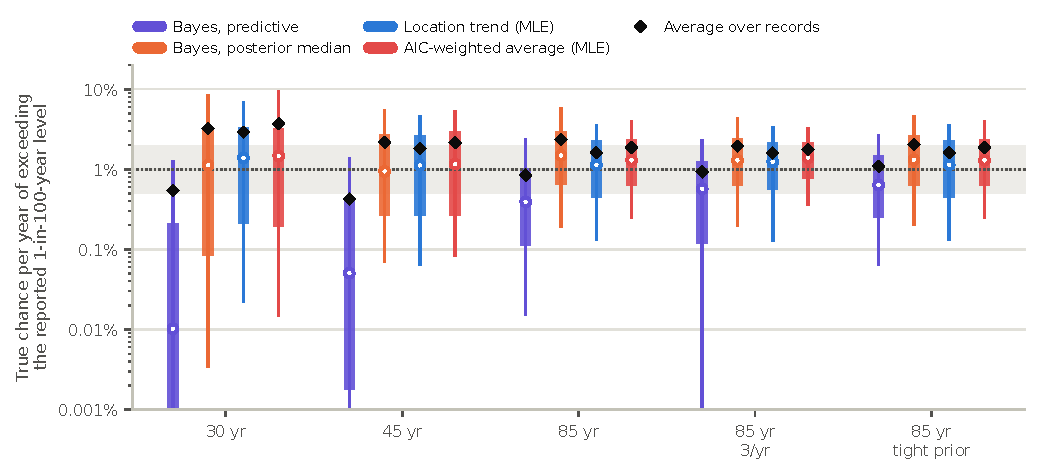
\includegraphics[width=\textwidth]{figures/pred_exceedance.pdf}
\caption{True chance of exceeding the reported 1-in-100-year level, over the records of the
standard cases: 10--90th percentiles (thin bar), 25--75th (thick bar), median (circle) and average
(diamond). The grey band is the factor-of-2 band around 1\%.}\label{fig:exceedance}
\end{figure}

\begin{itemize}
\item \textbf{The predictive level is usually too high.} Its median true exceedance is 0.39\% at 85
  years, 0.05\% at 45 and 0.01\% at 30. The other estimators are centred near 1\% (medians 0.9--1.5\%).
\item \textbf{It misses more often.} It is off by more than a factor of 2 in 68\% of records at
  85 years, 84\% at 45 and 92\% at 30, almost always by overstating. The posterior median misses in
  59\%, 70\% and 75\%, the location trend in 56\%, 69\% and 73\%.
\item \textbf{The dispersion is larger, and lopsided.} At 85 years the middle 80\% of its true
  exceedances runs from 0.015\% to 2.4\%, a factor of about 160; for the posterior median it is 0.19\%
  to 6\%, a factor of about 30. At 30 years, a tenth of predictive levels have essentially no chance of
  being exceeded in the simulated climate.
\item \textbf{The level itself is not far off; the probability is.} In the precipitation-like
  (gamma) records, the predictive 100-year depth is a median 8\% above the true depth at 85 years
  (10--90th percentile $-6\%$ to $+25\%$), 22\% above at 45 years and 31\% above at 30. Because the
  chance of exceedance falls steeply with depth in the far tail, an 8\% overstatement of the depth
  becomes a factor of 2.5 in the probability.
\item \textbf{Several values per year help, but only modestly.} Fitting the three largest
  (declustered) values of each year instead of the annual maximum cuts the share of records whose
  posterior leans heavy-tailed from 38\% to 14\% at 45 years and from 12\% to 8\% at 85 years
  (Table~\ref{tab:uncertainty}). The predictive level's median true exceedance rises from 0.05\% to
  0.2\% at 45 years and from 0.4\% to 0.6\% at 85, and its share missed falls from 84\% to 78\% and
  from 68\% to 60\%. But the other estimators gain about as much, so the predictive level still
  misses 7--16 points more often than the posterior median.
\end{itemize}

Table~\ref{tab:groups} breaks the 85-year results down by the kind of change and by distribution.
The predictive level overstates the risk more often than it understates it in every kind of case, including no
change at all. It does about as well as the posterior median only where the true change widens the
distribution or makes its upper tail heavier, so that the other estimators tend to understate the
risk: in the width cases (64\% missed, against 63\%) and when the spread and tail follow a rising
mean (68\% against 69\%). It does worst where the tail becomes lighter (79\% missed).

\begin{table}[H]
\centering\small\setlength{\tabcolsep}{3.5pt}
\caption{The predictive level at 85 years by kind of change and by distribution: median true
exceedance, shares (\%) understated and overstated by more than a factor of 2, and missed; right,
the share missed by other estimators on the same records.}\label{tab:groups}
\begin{tabular}{l r rrr r rrr}
\toprule
 & & \multicolumn{4}{c}{Bayes, predictive} & \multicolumn{3}{c}{Missed, others} \\
\cmidrule(lr){3-6}\cmidrule(lr){7-9}
Kind of change & records & median & under & over & \textbf{missed} & \shortstack{post.\\median} & \shortstack{loc.\\trend} & \shortstack{AIC\\avg.} \\
\midrule
No change & 400 & 0.5\% & 11 & 52 & \textbf{64} & 53 & 49 & 47 \\
Mean & 800 & 0.4\% & 14 & 54 & \textbf{67} & 57 & 52 & 45 \\
Width & 400 & 0.6\% & 19 & 46 & \textbf{64} & 63 & 54 & 54 \\
Tail & 300 & 0.2\% & 3 & 76 & \textbf{79} & 60 & 75 & 62 \\
Position (beta) & 100 & 0.2\% & 11 & 66 & \textbf{77} & 76 & 73 & 61 \\
Follows mean state & 700 & 0.6\% & 24 & 45 & \textbf{68} & 69 & 74 & 64 \\
Time-driven & 300 & 0.6\% & 24 & 47 & \textbf{71} & 68 & 71 & 65 \\
\midrule
Normal (standard cases) & 400 & 0.5\% & 15 & 50 & \textbf{65} & 60 & 50 & 46 \\
Gamma (standard cases) & 500 & 0.4\% & 11 & 56 & \textbf{67} & 53 & 50 & 47 \\
Student-t (standard cases) & 500 & 0.4\% & 9 & 55 & \textbf{64} & 50 & 56 & 46 \\
Beta (standard cases) & 600 & 0.3\% & 15 & 60 & \textbf{75} & 70 & 66 & 60 \\
\bottomrule
\end{tabular}

\end{table}

\section{The average versus a single record}\label{sec:average}

The predictive level does what it is built to do on average: the true chance of exceeding it,
averaged over records, is 0.85\% at 85 years (0.43--0.55\% at 30--45 years), the closest to 1\% of
the estimators we tested, alongside the posterior mean; the posterior median and the
maximum-likelihood fits average 1.6--3.7\% (diamonds in Figure~\ref{fig:exceedance}).
But the average is carried by a minority of records in which the level is too low, while in the
typical record it is far too high.

This is the familiar gap between the average and the typical value of a skewed quantity. For a
risk taker who writes many independent contracts and cares only about the expected total, the
average is the relevant number, and by that standard the predictive level is well calibrated or
conservative. For a single contract, location or portfolio exposed to one climate, the typical
record is more relevant, and there the predictive level usually implies a risk several times
higher than the true one. Climate risks at nearby locations are strongly correlated, and a model and
prior applied in the same way everywhere will err in the same direction everywhere, so the
diversification that would make the average relevant is limited.

A Bayesian predictive distribution is calibrated in this average sense when the true climates are
drawn from the prior. Our synthetic climates are not drawn from the authors' prior: the GEV shape
of their annual maxima is at most about 0.2 (the Student-$t$ case), whereas the prior allows $\xi$
up to 2.1, and above $\xi=1$ even the mean of the distribution is infinite. To the extent that real
rainfall extremes have lighter tails than the prior allows, the same overstatement should be
expected in real records.

\section{Pricing cover with a known 1\% risk}\label{sec:price}

Figure~\ref{fig:price} turns the question around: for the level whose true chance of being
exceeded is exactly 1\% in the final year, what chance does each model assign? That chance is the
pure premium rate the model would charge for cover triggered at that level.

\begin{figure}[H]
\centering
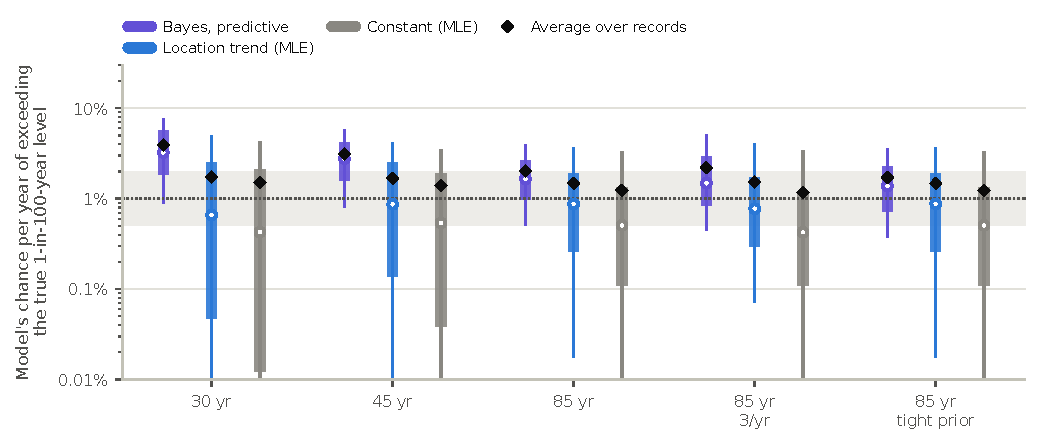
\includegraphics[width=\textwidth]{figures/pred_price.pdf}
\caption{Each model's chance of exceeding the true 1-in-100-year level of the final year, over the
records of the standard cases (percentiles as in Figure~\ref{fig:exceedance}). The grey band is a
factor of 2 around the true 1\%.}\label{fig:price}
\end{figure}

\begin{itemize}
\item \textbf{The predictive model charges too much, but rarely too little.} Its median rate is 1.7\%
  at 85 years, 2.8\% at 45 and 3.2\% at 30. It charges less than 0.5\% in only 4--10\% of records
  and less than 0.1\% almost never; it charges more than 2\% in 40\% of records at 85 years and in
  67--72\% at 30--45 years.
\item \textbf{A trend fit is right on average but often dangerously low.} The location-trend
  maximum-likelihood fit has a median rate of 0.7--0.9\%, but charges less than 0.5\% in 36--45\% of
  records and less than 0.1\% in 16--28\%: in those records the cover would be priced at a tenth or
  less of its true cost.
\item The predictive approach therefore trades frequent and large over-pricing for protection
  against severe under-pricing. Whether that is a good trade is a question about risk preferences;
  the point here is that the loading it implies is large, varies by a factor of several from one
  record to the next, and is set mainly by the prior (Section~\ref{sec:prior}).
\end{itemize}

\section{Where the uncertainty comes from}\label{sec:sources}

\subsection{The posterior's own spread}

Figure~\ref{fig:anatomy} shows one typical precipitation-like record of 85 years with no change.
Left: each grey curve is the chance of exceeding a given level under one posterior draw. The draws
fan out in the tail. The predictive curve (violet) is their average; it lies above most of the
draws because the few heavy-tailed ones dominate the average in the far tail. Right: the
distribution over draws of the chance of exceeding the predictive level. By construction it
averages 1\%, but the median draw gives 0.40\%, close to the truth (0.48\%), and the top 5\% of
draws carry a third of the average.

\begin{figure}[H]
\centering
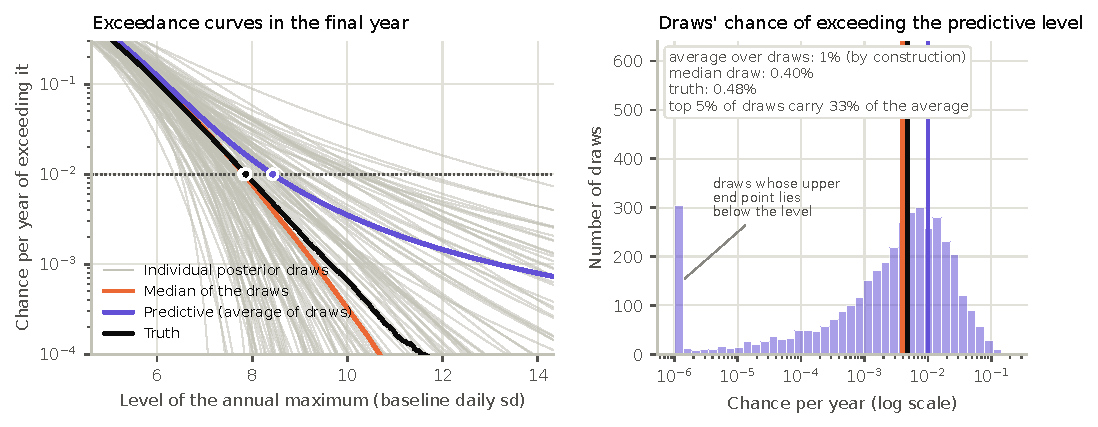
\includegraphics[width=\textwidth]{figures/pred_anatomy.pdf}
\caption{One record (precipitation-like distribution, 85 years, no change; the record whose
predictive level has the median true exceedance of that case). Left: exceedance curves of 120
posterior draws (grey), their median (orange), their average, i.e.\ the predictive curve (violet),
and the truth (black); dots mark the levels with a 1\% chance. Right: the draws' chance of
exceeding the predictive level (log scale; draws that put it at or below $10^{-6}$ are gathered in
the leftmost bar).}\label{fig:anatomy}
\end{figure}

Table~\ref{tab:uncertainty} summarises this over all records. The posterior is honest about its
uncertainty: the true chance lies within the draws' 5--95\% range in 96--100\% of records. But the
range is very wide, from essentially 0 to about 5\%, so the single number hides a very wide spread
of beliefs. ``Dominated by a few draws'' is accurate in a specific sense: the top 5\% of draws
carry 38\% (85 years) to 52\% (30 years) of the 1\%, and the effective number of draws that
determine the average is 13--21\% of the total.

\begin{table}[H]
\centering\small\setlength{\tabcolsep}{3pt}
\caption{Uncertainty measures of the predictive level, standard cases. Left: the median over
records of the 5th, 50th and 95th percentiles over draws of each draw's chance of exceeding the
predictive level. \emph{Heavy-tailed}: the share of records in which more than 5\% of the draws
have $\xi>0.5$. \emph{Truth inside}: how often the true chance lies within the draws' 25--75\% and
5--95\% ranges. \emph{Top 5\%}: the share of the 1\% carried by the top 5\% of draws (median over
records). \emph{Monte Carlo}: the typical error of the exceedance probability with 4,000 draws, as
a multiplicative factor.}\label{tab:uncertainty}
\begin{tabular}{l rrr r rr r r}
\toprule
 & \multicolumn{3}{c}{\shortstack{Draws' chance of\\exceeding the level}} & & \multicolumn{2}{c}{\shortstack{Truth\\inside}} & & \\
\cmidrule(lr){2-4}\cmidrule(lr){6-7}
Design & 5\% & median & 95\% & \shortstack{heavy-\\tailed} & 50\% & 90\% & \shortstack{top\\5\%} & \shortstack{Monte\\Carlo} \\
\midrule
30 yr & 0.00\% & 0.00\% & 5.8\% & 53\% & 64\% & 96\% & 52\% & $\times$1.11 \\
45 yr & 0.00\% & 0.04\% & 5.4\% & 38\% & 69\% & 100\% & 47\% & $\times$1.10 \\
85 yr & 0.00\% & 0.2\% & 4.6\% & 12\% & 67\% & 98\% & 38\% & $\times$1.06 \\
45 yr, 3/yr & 0.00\% & 0.2\% & 4.5\% & 14\% & 69\% & 98\% & 35\% & $\times$1.06 \\
85 yr, 3/yr & 0.00\% & 0.4\% & 3.9\% & 8\% & 65\% & 97\% & 27\% & $\times$1.04 \\
85 yr, indep. days & 0.00\% & 0.2\% & 4.6\% & 17\% & 61\% & 98\% & 38\% & $\times$1.06 \\
45 yr, tight prior & 0.00\% & 0.3\% & 4.4\% & 18\% & 54\% & 97\% & 34\% & $\times$1.06 \\
85 yr, tight prior & 0.00\% & 0.5\% & 3.8\% & 4\% & 57\% & 96\% & 28\% & $\times$1.03 \\
\bottomrule
\end{tabular}

\end{table}

\subsection{The tail shape}

Which records are overstated most? Those whose posterior leans towards heavy tails
(Figure~\ref{fig:xi}). The true GEV shape of the annual maxima in our climates ranges from about
$-0.25$ (bounded) to about $+0.17$ (Student-$t$); with 30--45 years of data the posterior mean of $\xi$
is often well above that, and every positive shift in $\xi$ raises the predictive level steeply.
At 30 years, records with a posterior mean $\xi$ above about 0.2 have predictive levels with
essentially no chance of being exceeded.

\begin{figure}[H]
\centering
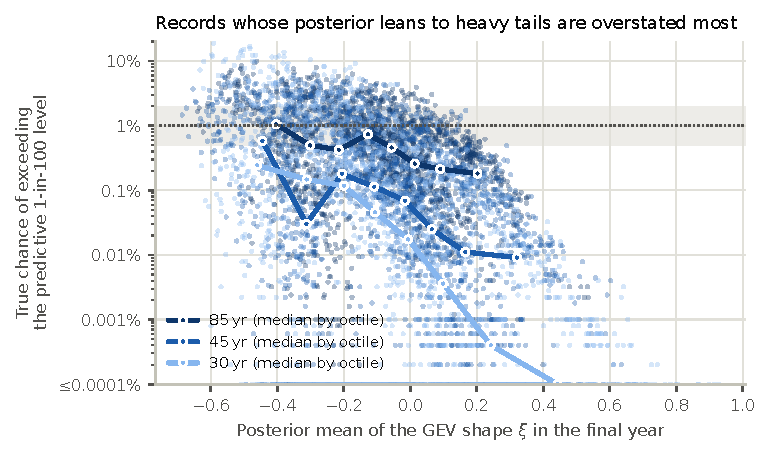
\includegraphics[width=0.75\textwidth]{figures/pred_xi.pdf}
\caption{True chance of exceeding the predictive level against the posterior mean of the GEV
shape $\xi$ in the final year, standard cases at 30, 45 and 85 years (one dot per record; lines:
medians within octiles of $\xi$).}\label{fig:xi}
\end{figure}

\subsection{The prior}\label{sec:prior}

The predictive level is ``unique'' only for a given prior, and the prior matters a great deal.
Shrinking the prior scales of the random walks from the authors' values (1, 0.5, 0.5) to 0.25
changes nothing about the data, but:
\begin{itemize}
\item at 85 years the share missed falls from 68\% to 57\% (now within 1 point of the posterior
  median and the location trend), and the median true exceedance rises from 0.39\% to 0.64\%;
\item at 45 years the share missed falls from 84\% to 74\% and the median true exceedance rises from
  0.05\% to 0.24\%; record by record the true exceedance of the predictive level rises by a median
  factor of 2.8 (85 years: 1.6);
\item in the cases where the spread and tail follow a rising mean, at 85 years, the predictive level
  with the tight prior becomes the best estimator we tested, missing in 55\% of records against 64\%
  for the Akaike-weighted average and 69\% for the posterior median.
\end{itemize}
We varied only the random-walk scales. The prior on $\xi$ itself, and its upper limit of 2.1, are
likely to matter as much, because the overstatement comes from heavy-tailed draws.

\subsection{Monte Carlo error}

Splitting each fit's 4,000 draws into its four chains, the predictive level's chance of being
exceeded changes by a typical factor of 1.06 at 85 years and 1.10--1.11 at 30--45 years (90th
percentile 1.16--1.55). With the authors' 40,000 draws these factors would shrink by about
$\sqrt{10}$. Monte Carlo error accounts for well under 1\% of the variance of the error in the
log exceedance probability (0.03--0.11\%): the dominance of a few draws is a property of the posterior, not of
the number of draws.

\section{Ambiguity in the climate, or in the inference?}\label{sec:ambiguity}

The argument for the predictive approach is that possible non-stationarity, combined with possibly
long tails, makes the climate distribution genuinely ambiguous, and that the high and volatile
estimates of catastrophic risk reflect that ambiguity. The synthetic records let us separate the
two parts, because in the no-change cases nothing is changing and the true tail is at most moderately heavy
($\xi\lesssim0.2$):

\begin{table}[H]
\centering\small
\caption{No-change cases only (400 records per design): true chance of exceeding the reported
1-in-100-year level (median and 10--90th percentiles) and the share missed by more than a factor of
2.}\label{tab:null}
\begin{tabular}{l rrr rrr}
\toprule
 & \multicolumn{3}{c}{Bayes, predictive} & \multicolumn{3}{c}{Missed $>2\times$} \\
\cmidrule(lr){2-4}\cmidrule(lr){5-7}
Design & median & 10\% & 90\% & predictive & post.\ median & loc.\ trend \\
\midrule
30 yr & 0.02\% & 0.00\% & 1.35\% & 89 & 73 & 73 \\
45 yr & 0.08\% & 0.00\% & 1.46\% & 80 & 65 & 66 \\
85 yr & 0.47\% & 0.04\% & 2.31\% & 64 & 53 & 49 \\
85 yr, tight prior & 0.68\% & 0.12\% & 2.30\% & 52 & 48 & 49 \\
\bottomrule
\end{tabular}
\end{table}

With no change at all, the predictive level is as high and as dispersed as in the cases with
change. So most of the ambiguity is produced by the inference: a few decades of annual maxima
cannot rule out a heavy tail, the prior allows one, and averaging probabilities over the posterior
turns that possibility into a high level. That is a legitimate feature of a Bayesian learner's
beliefs, and it is real ambiguity for someone who must act on a short record. But it would be
present in a stationary climate, it shrinks with record length roughly as the tail becomes
identifiable, and its size is governed by prior choices that the data cannot check. It is not, by
itself, evidence that the climate's extremes are changing or are heavy-tailed.

\section{Suggestions for practice}\label{sec:suggest}

\begin{enumerate}
\item \textbf{Report the spread of beliefs, not only the average.} Alongside the predictive level,
  report the posterior distribution of the chance of exceeding it, for example the median draw and
  a 90\% range (in our records typically $\sim$0.2\% and 0--5\% at 85 years). That makes clear that
  ``1\%'' is an average over beliefs ranging from negligible to several times the target.
\item \textbf{Show prior sensitivity.} Refit with tighter random-walk scales and a more
  informative prior on $\xi$ (or a lower upper bound), and report how the level and the implied
  premium move. In our records, the random-walk scales alone change the typical true exceedance
  by a factor of 1.6 (85 years) to 2.8 (45 years).
\item \textbf{Benchmark against a stationary climate.} Fit the model to synthetic stationary
  records of the same length and similar distribution. The spread of predictive levels obtained
  there is the ambiguity that comes from the inference alone.
\item \textbf{Compare with simple fits.} If the predictive level is far above both a constant and a
  trend maximum-likelihood fit, the difference comes from the posterior's heavy-tailed draws, and
  should be justified on other grounds (physical or regional knowledge of the tail).
\item \textbf{Bring in more information on the tail.} Pooling the shape parameter across nearby
  stations (regional frequency analysis), or using several values per year, constrains $\xi$
  better than a single annual-maximum record, and the overstatement shrinks as $\xi$ is pinned down.
  In our records, three values per year from 45 years constrained $\xi$ about as well as 85 years
  of annual maxima, but the predictive level still missed in 78\% of records against 68\%; at
  85 years it did slightly less than the tight prior (60\% missed against 57\%). Pooling across
  stations is likely to do more.
\item \textbf{Separate the risk margin from the estimate.} The predictive approach builds a loading
  for ambiguity into the estimate through the prior. If a margin for ambiguity is wanted, it may be
  clearer to estimate the risk with a well-calibrated central estimate and add an explicit,
  stated margin, so that the margin is a decision rather than a by-product of the prior.
\end{enumerate}

\section{Caveats}\label{sec:caveats}

\begin{itemize}
\item Synthetic climates: four distributions and a limited set of changes. Real rainfall extremes
  may have heavier tails than ours; if their true $\xi$ is clearly positive, the predictive level
  will overstate less, and the other estimators will understate more.
\item One model, with the authors' priors and one alternative for the random-walk scales. We did not
  vary the prior on $\xi$.
\item We scored the final year of each record (a ``nowcast''); a forecast for future years would add
  the uncertainty of extrapolating the random walks.
\item 4,000 draws per fit rather than the authors' 40,000 (shown above to matter little), and, as in
  the authors' replication code, no importance-sampling correction for the extended-support
  likelihood (whose weights they report to be essentially 1).
\item 100 records per case. Pooled shares are measured to about $\pm1$ percentage point, and
  differences between estimators on the same records to about $\pm1.5$.
\end{itemize}

\appendix
\section{Results at 30 years by kind of change}

\begin{table}[H]
\centering\small\setlength{\tabcolsep}{3.5pt}
\caption{As Table~\ref{tab:groups}, at 30 years.}
\begin{tabular}{l r rrr r rrr}
\toprule
 & & \multicolumn{4}{c}{Bayes, predictive} & \multicolumn{3}{c}{Missed, others} \\
\cmidrule(lr){3-6}\cmidrule(lr){7-9}
Kind of change & records & median & under & over & \textbf{missed} & \shortstack{post.\\median} & \shortstack{loc.\\trend} & \shortstack{AIC\\avg.} \\
\midrule
No change & 400 & 0.02\% & 7 & 82 & \textbf{89} & 73 & 73 & 74 \\
Mean & 800 & 0.01\% & 9 & 84 & \textbf{92} & 75 & 69 & 72 \\
Width & 400 & 0.02\% & 10 & 81 & \textbf{91} & 77 & 76 & 79 \\
Tail & 300 & 0.01\% & 3 & 92 & \textbf{95} & 73 & 79 & 74 \\
Position (beta) & 100 & 0.00\% & 7 & 88 & \textbf{95} & 80 & 76 & 77 \\
Follows mean state & 700 & 0.01\% & 9 & 78 & \textbf{87} & 80 & 83 & 82 \\
Time-driven & 300 & 0.01\% & 9 & 81 & \textbf{90} & 78 & 83 & 81 \\
\midrule
Normal (standard cases) & 400 & 0.01\% & 8 & 82 & \textbf{90} & 75 & 72 & 76 \\
Gamma (standard cases) & 500 & 0.02\% & 7 & 84 & \textbf{91} & 72 & 70 & 73 \\
Student-t (standard cases) & 500 & 0.04\% & 7 & 84 & \textbf{91} & 73 & 70 & 69 \\
Beta (standard cases) & 600 & 0.00\% & 8 & 87 & \textbf{95} & 79 & 79 & 80 \\
\bottomrule
\end{tabular}

\end{table}

\section{Reproducing these results}

{\sloppy
The Bayesian fits are rerun with \texttt{python scripts/stage\_c.py --replay}, which refits every
saved scenario with its original seeds and settings and adds the predictive quantiles, the
per-chain values, the spread of the draws' exceedance probabilities and the final-year posterior
draws (written to \texttt{data/output/stage\_c\_pred}; about 20 hours on 14 cores). The posterior
medians and means reproduce the earlier runs to within $3\times10^{-6}$. The tables, figures and
numbers of this note come from \texttt{python scripts/predictive\_note.py}, which also writes the
summary tables \texttt{predictive\_headline.csv}, \texttt{predictive\_uncertainty.csv} and
\texttt{predictive\_rain\_ratio.csv} in \texttt{data/results}.\par}

\end{document}
